\chapter{Topology of the $D^0 \rightarrow \pi+K$ decay}
\label{ch:d0_top}

This chapter begins our discussion of the work conducted for this thesis. Here, we first discuss the topology of the $D^0\rightarrow\pi+K$ decay, which we use to distinguish true $D^0$ signals from background. We introduce the topological variables in Ch. \ref{sec.d0_intro}-\ref{sec:def_top_vars}, then examine the distributions of these variables and their dependence on $D^0$ kinematics in Ch. \ref{sec.d0_kinematics}. Finally in Ch. \ref{sec.d0_strategy}, we outline our plan for utilizing these topological distributions in our $D^0$ analysis.

All of the data used in this thesis come from PYTHIA-8 simulations of $ep$ collisions, provided by the ePIC Collaboration (ref. in Appendix \ref{app.samples}).

%------------------------------------------------------
\section{$D^0$ production and decay}
\label{sec.d0_intro}

In high energy experiments, such as electron-proton collisions at the EIC, charm quarks are produced and hadronize into heavy flavor particles. $D^0$-mesons, containing one charm quark and one up quark, are the lightest and thus most abundant of these heavy flavor particles. However, the $D^0$ cannot be directly detected due to their short lifetime and neutral electric charge. Thus, we must reconstruct the $D^0$ from the tracks left by its decay daughters. In this analysis, we focus on the $D^0 \rightarrow \pi+K$ decay channel, in which a $D^0$-meson decays into a pair of oppositely charged pion and kaon daughters, either $\pi^++K^-$ or $\pi^-+K^+$. Fig. \ref{f.ep_d0_pik} provides a cartoon illustration to summarize this channel of $D^0$ production and decay.
%
\begin{figure}[h!]
    \centering
    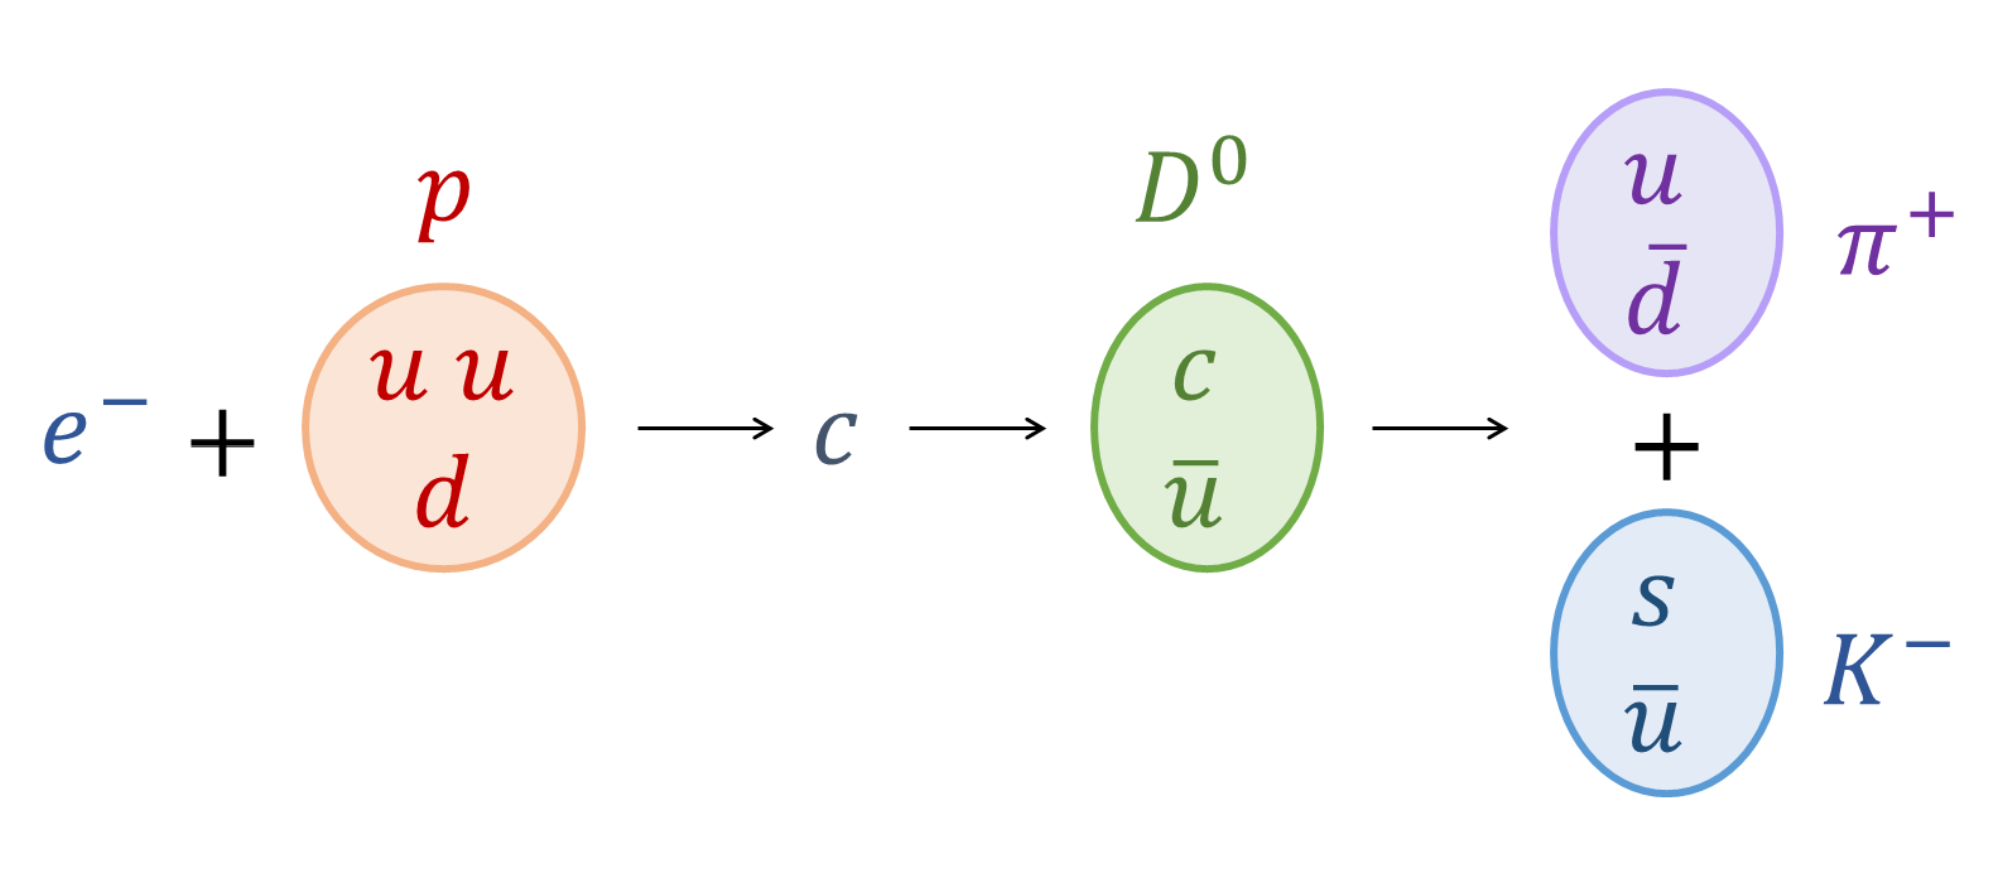
\includegraphics[width=0.7\linewidth]{gallery/D0_topology/ep_d0_pik.png}
    \caption{Production and decay of a $D^0$-meson in an $ep$ collision.}
    \label{f.ep_d0_pik}
\end{figure}
%

A major challenge in reconstructing $D^0$-mesons is identifying the correct $\pi K$ pairs. Pions and kaons, being the lightest hadrons, are constantly produced through a variety of processes. In contrast, due to the high mass of the charm quark (1.27 GeV/c$^2$), heavy flavor particles like the $D^0$ are rarely produced. Consequently, most of the measured pions and kaons do not originate from a $D^0$ decay, and random $\pi K$ combinations form a large {\it background} that can obscure the true $D^0$ signals we are looking for.

Fortunately, the $D^0\rightarrow \pi+K$ decay occurs with a specific {\it topology}, or geometric pattern, which we can leverage to distinguish $D^0$ signals from background. If we measure the topological variables associated with each reconstructed $\pi K$ pair, we can expect the distributions of true $D^0$-decayed pairs to look different from those of random background pairs. The strategy then is to apply a set of {\it topological cuts}, or selection criteria on the topological variables, to help separate the signal and background candidates. 

%------------------------------------------------------
\section{Topological variables defined}
\label{sec:def_top_vars}

Fig. \ref{f.d0_decay_diagram} depicts the particle trajectories associated with $D^0 \rightarrow \pi+K$ in the transverse plane, forming the two-dimensional decay topology. The {\it primary vertex} marks the location at which the $ep$ collision occurs and the $D^0$ is produced. The $D^0$ travels for some distance and then decays at the $D^0$ decay vertex, a type of {\it secondary vertex}. The pion and kaon daughters then travel away from the decay vertex, their paths bent in opposite directions due to the presence of a magnetic field. Passing through the detectors, they leave hits that are fitted into tracks (represented by the solid blue curves.)

%
\begin{figure}[h!]
    \centering
    \includegraphics[width=0.6\linewidth]{gallery/D0_topology/d0_decay.png}
    \caption{$D^0\rightarrow \pi^+ + K^-$ decay in the transverse plane. Solid blue lines indicate the directly detected pion and kaon tracks. Dashed lines indicate reconstructed particle trajectories. Figure from the STAR Collaboration \cite{STAR}.}
    \label{f.d0_decay_diagram}
\end{figure}
%

Based on knowledge of the magnetic field strength and particle momenta, we can extrapolate the detected $\pi K$ tracks backward in space and time (dashed curves), forming a {\it helix} trajectory for each particle. (The transverse trajectories are circular due to the magnetic field, but motion in the $z$-direction is constant. Thus in three-dimensions, the particle paths are helical.) We then measure the {\it distance of closest approach (DCA)} between the $\pi K$ pair (${\rm DCA}_{12}$), defined as the perpendicular distance between the two helices, and reconstruct the $D^0$ decay vertex at the midpoint. The primary vertex is reconstructed similarly, but using particles originating from the initial $ep$ collision. Using conservation of momentum, we can also reconstruct the $D^0$ momentum vector $\overrightarrow{P}$. Since the $D^0$ is electrically neutral, its trajectory is a straight line in the direction of $\overrightarrow{P}$.

Following a previous $D^0$ analysis by the STAR Collaboration \cite{STAR}, we use the following topological variables to characterize the $D^0\rightarrow\pi+K$ decay:
\begin{itemize}
    \item ${\rm DCA}_{12}$: distance of closest approach between $\pi K$ pair
    \item ${\rm DCA_\pi}$: distance of closest approach of $\pi$ to primary vertex
    \item ${\rm DCA_K}$: distance of closest approach of $K$ to primary vertex
    \item ${\rm DCA_{D0}}$: distance of closest approach of $D^0$ (or $\overrightarrow P$) to primary vertex
    \item Decay Length: distance between primary vertex and secondary vertex
    \item $\theta$: angle between $\overrightarrow{P}$ and the line connecting primary vertex to secondary vertex
\end{itemize}
Note that Fig. \ref{f.d0_decay_diagram} visualizes the decay topology projected onto the transverse plane, so all variables in the picture are technically the two-dimensional components, ${\rm DCA}_{{\rm \pi}{(xy)}}$,  ${\rm DCA}_{{\rm K}{(xy)}}$, $\theta_{xy}$, etc.


%------------------------------------------------------
\section{Dependence of topological variables on $D^0$ kinematics}
\label{sec.d0_kinematics}

%--------------------------
\subsection{Kinematic variables: rapidity ($y$) and transverse momentum ($p_T$)}
\label{sec:dep_of_top_dists}
%
\begin{figure}[h!]
    \centering
    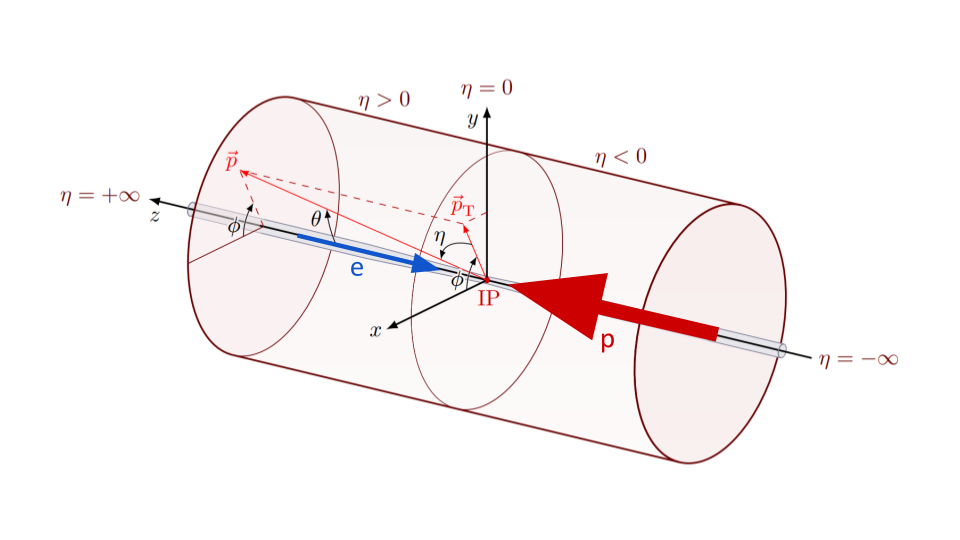
\includegraphics[width=0.65\linewidth]{gallery/D0_topology/coordinates.png}
    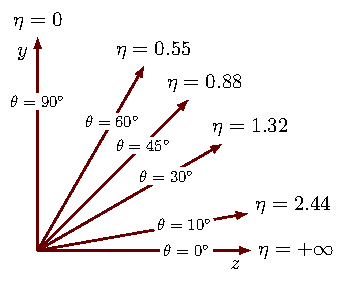
\includegraphics[width=0.3\linewidth]{gallery/D0_topology/pseudorapidity.pdf}
    \caption{Coordinate system for collider experiments. The red arrow indicates the proton beam, and the blue arrow indicates the electron beam, both pointing in the particles' direction of travel. Figures adapted from \cite{tikz}.}
    \label{f.coordinates}
\end{figure}
%
In high energy collisions, particles are accelerated to relativistic speeds. Thus, we describe their motion using a ``relativistic version" of velocity known as {\it rapidity}  (see Appendix \ref{sec.relativity}), defined
\begin{align}
    y \equiv \tanh^{-1}(v_z)\equiv \frac{1}{2}\ln \left[ \frac{E+p_z}{E-p_z} \right] \ , \label{eqn.rapidity}
\end{align}
where $v_z$ is the velocity of the particle, $E$ is its total energy, and $p_z$ is its momentum. By convention, we take the particles' direction of motion to be along the $z$-axis, which defines the beam axis. In $ep$ collisions, we define the proton beam to travel toward the $(+z)$-direction, or the forward direction, and the electron beam to travel toward the $(-z)$-direction, or the backward direction.

In high energy experiments, we measure the closely related {\it pseudorapidity},
\begin{equation}
    \eta \equiv -\ln\left[\tan\left(\frac{\theta}{2}\right) \right] \equiv \frac{1}{2}\ln \left[\frac{|\mathbf{p}|+p_z}{|\mathbf{p}|-p_z} \right] \ ,
\end{equation}
where $\theta$ is the polar angle with respect to the beam axis, and $\mathbf{p}$ is the three-dimensional momentum vector of a particle. The pseudorapidity has a nice geometric interpretation, as depicted in Fig. \ref{f.coordinates}. Particles with $\eta \approx 0$ are detected in the central region of the collision and have $p_L\approx0$. Particles with $\eta>0$ are found in the forward region while particles with $\eta<0$ are found in the backward region, with larger $|\eta|$ being closer to the ends of the collision region and corresponding to larger $|p_z|$. For particles traveling near the speed of light, $E\gg m$. They become near-massless, $|\mathbf{p}|\approx E$, and thus $\eta \approx y$. In this thesis, we use the terms ``pseudorapidity" and ``rapidity" interchangeably.

{\color{brown} Define/introduce transverse momentum.}

%
\begin{figure}[h!]
    \centering
    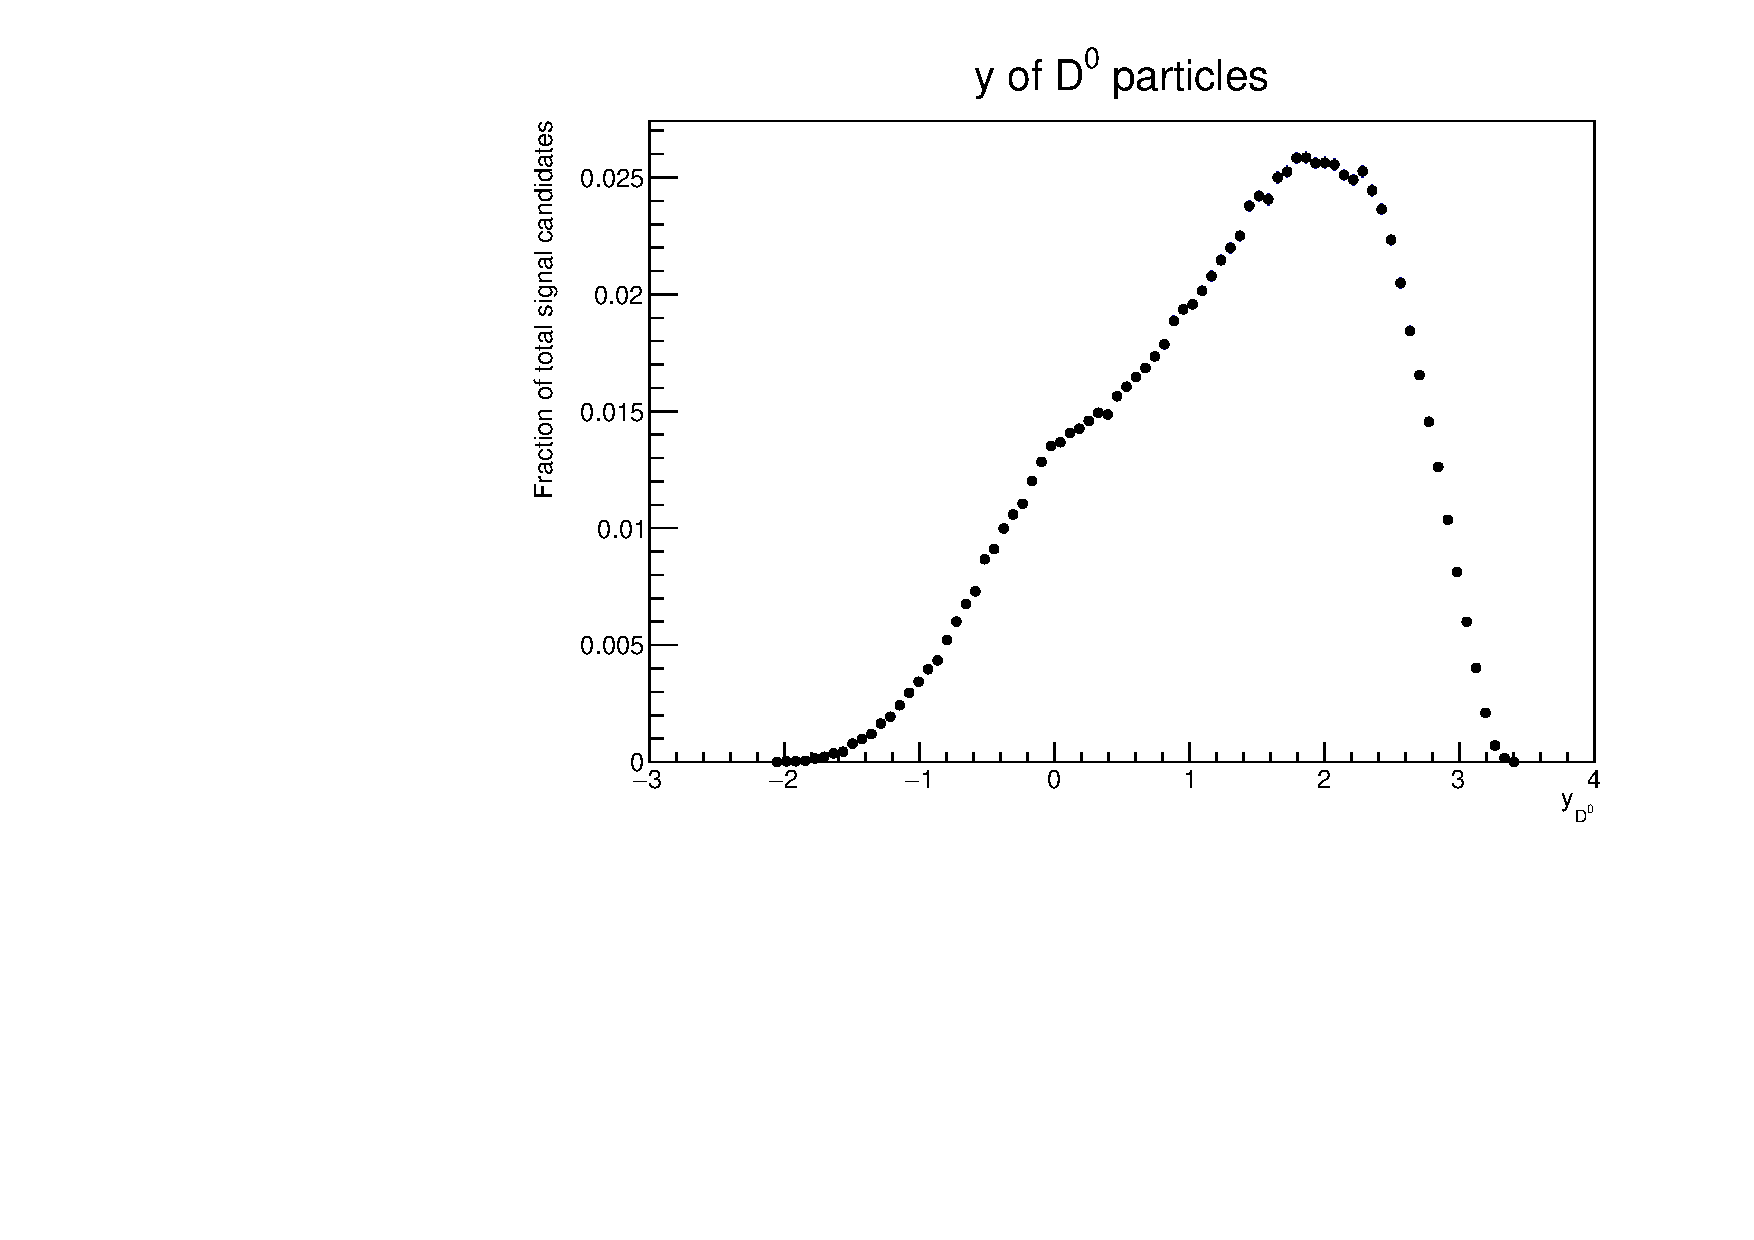
\includegraphics[width=0.45\linewidth]{gallery/D0_topology/D0_y.pdf}
    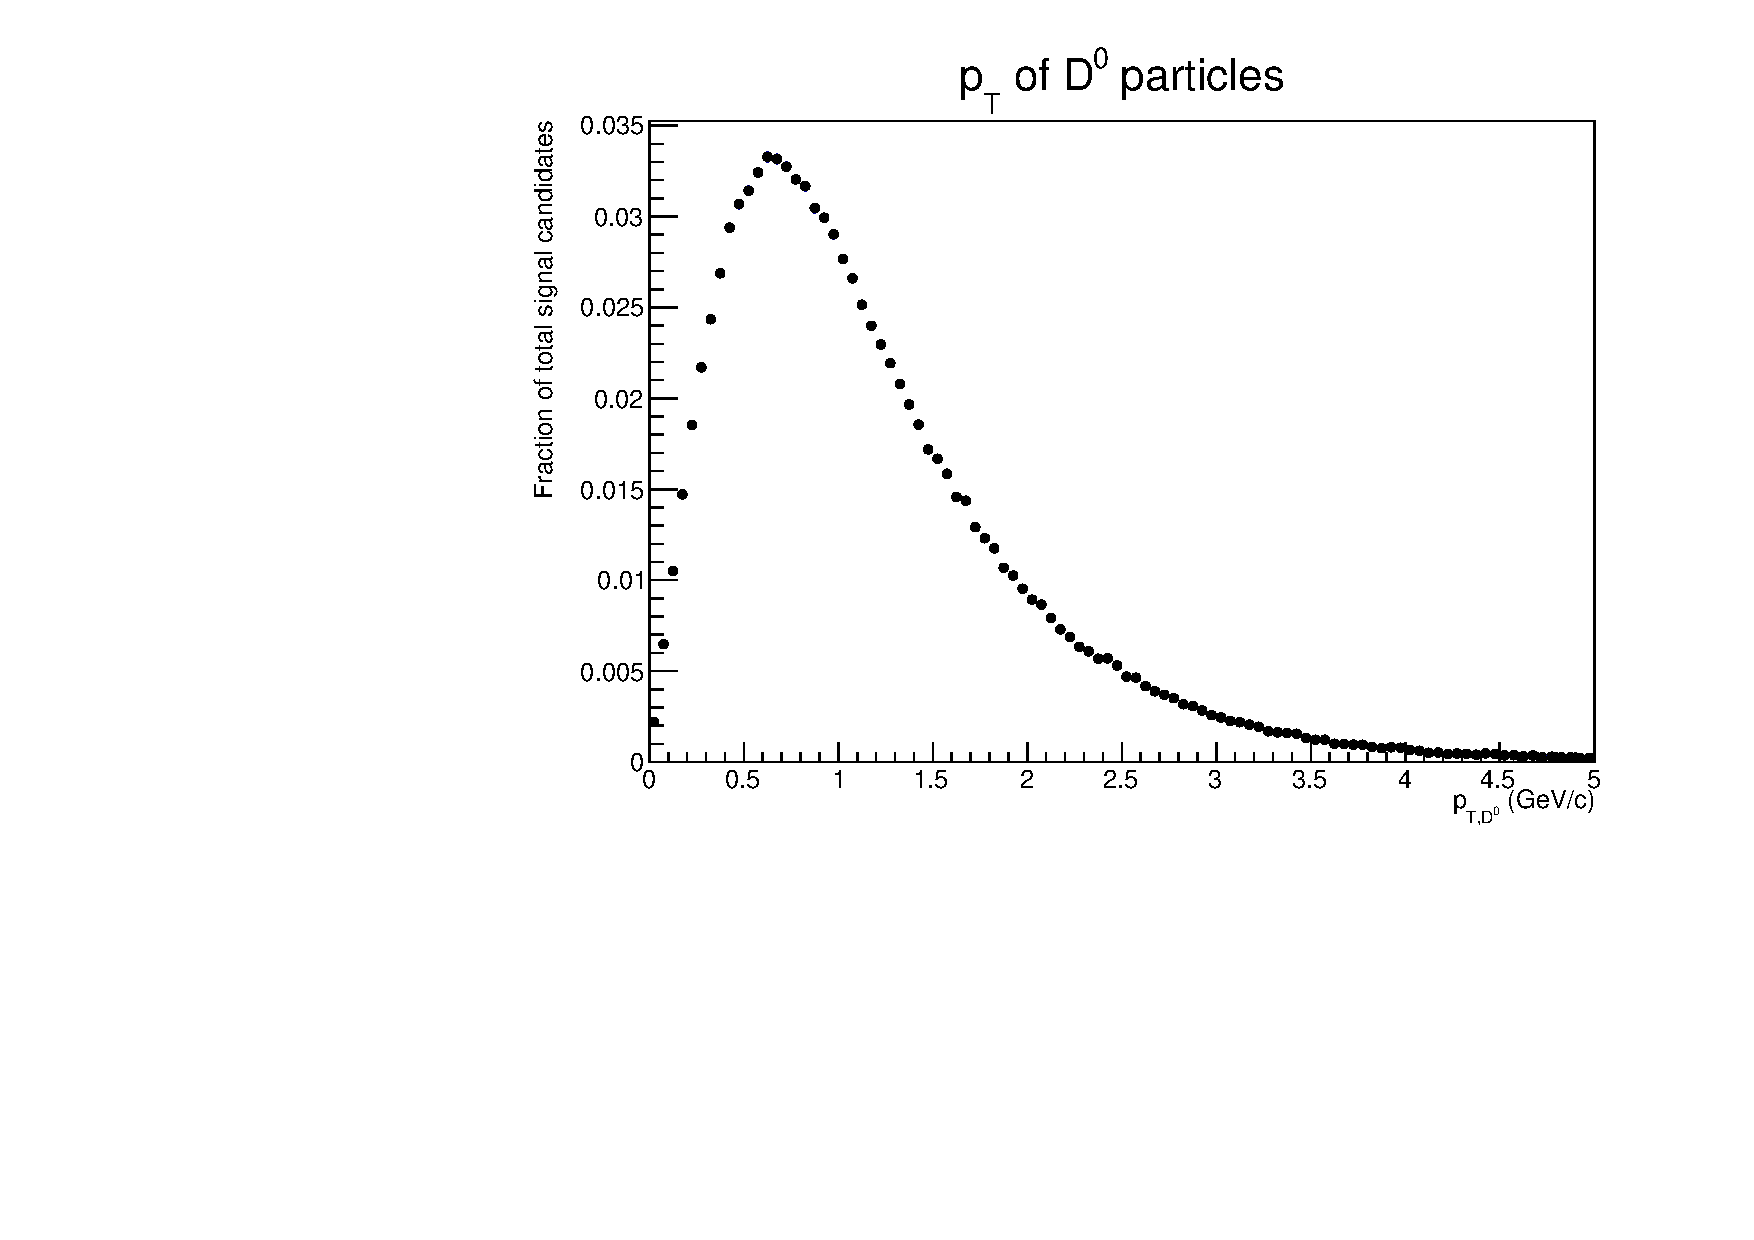
\includegraphics[width=0.45\linewidth]{gallery/D0_topology/D0_pT.pdf}
    \caption{Rapidity ($y$) and transverse momentum ($p_T$) distributions of reconstructed $D^0$-mesons in simulated $ep$ collisions with $Q^2>1~\text{GeV}^2$.}
    \label{f.y_pT}
\end{figure}
%
Fig. \ref{f.y_pT} shows the $y$ and $p_T$ distributions of $D^0$-mesons produced in simulated $ep$ collisions with $Q^2>1$. Here, it is interesting to see that the $y$ distribution is skewed toward the forward (positive) side, reflecting the asymmetry of the collision system. Because the proton has much more mass ($0.938~{\rm GeV/c^2}$) than the electron ($0.511~{\rm GeV/c^2}$), the net momentum is in the proton's direction of motion. Thus, most particles are produced at forward rapidity, with $y>0$ and $\eta>0$. The $p_T$ distribution peaks near $0.7~{\rm GeV/c}$ then falls off, with relatively few $D^0$-mesons exhibiting $p_T>2~{\rm GeV/c}$.

% We divide the analysis into  mid-rapidity $-1<y~(\eta)<1$ and forward rapidity $1<y~(\eta)<3$. However, the shapes of the $D^0 \rightarrow \pi+K$ topological distributions (as we will see in the next section \ref{sec.top_y_pt_slices}).

% Fig. \ref{f.y_pT} also shows the $p_T$ distributions of the $D^0$-mesons, which peaks around 0.7 GeV/c. High-$p_T$ $D^0$-mesons, which results in high-$p_T$ pions and kaons, travel with straighter trajectories and are therefore more easily reconstructed.  

%--------------------------
\subsection{$D^0$ topological distributions in various $y$ and $p_T$ slices}
\label{sec.top_y_pt_slices}

Let us first consider how we might expect the $D^0\rightarrow\pi+K$ topology to depend on $y$ and $p_T$ of the $D^0$. From a physics perspective, the $D^0$ momentum affects its lifetime and the trajectories of its $\pi K$ daughters. According to special relativity, $D^0$-mesons with a larger momentum (or velocity) experience greater time dilation, which means that they travel farther before decaying. Furthermore, the $\pi K$ daughters will also have larger momenta, which means that their trajectories are less bent by the magnetic field. Thus, we can expect higher $p_T$ to be correlated with larger decay length and smaller ${\rm DCA_\pi}$ and ${\rm DCA_K}$.

In addition to the physics, there are also reconstruction effects at play. In general, because higher $p_T$ tracks are straighter, they can be fitted and extrapolated with better precision. As for rapidity, detector performance tends to be better at mid-$y$ (mid-$\eta$), far away from the particle beams, so reconstruction is also better at mid-rapidity compared to forward and backward rapidity. Thus, high $p_T$ and mid-$y$ yield the most accurate and precise results. For the $D^0 \rightarrow\pi+K$ topology, this could mean smaller ${\rm DCA}_{12}$, ${\rm DCA_{D0}}$, and $\theta$ in these regions. (If reconstruction were perfect, then these values would be 0, since the $D^0$ should originate at the primary vertex and decay at the decay vertex, where the pion and kaon then originate together.)
%
\begin{figure}[h!]
    \centering
    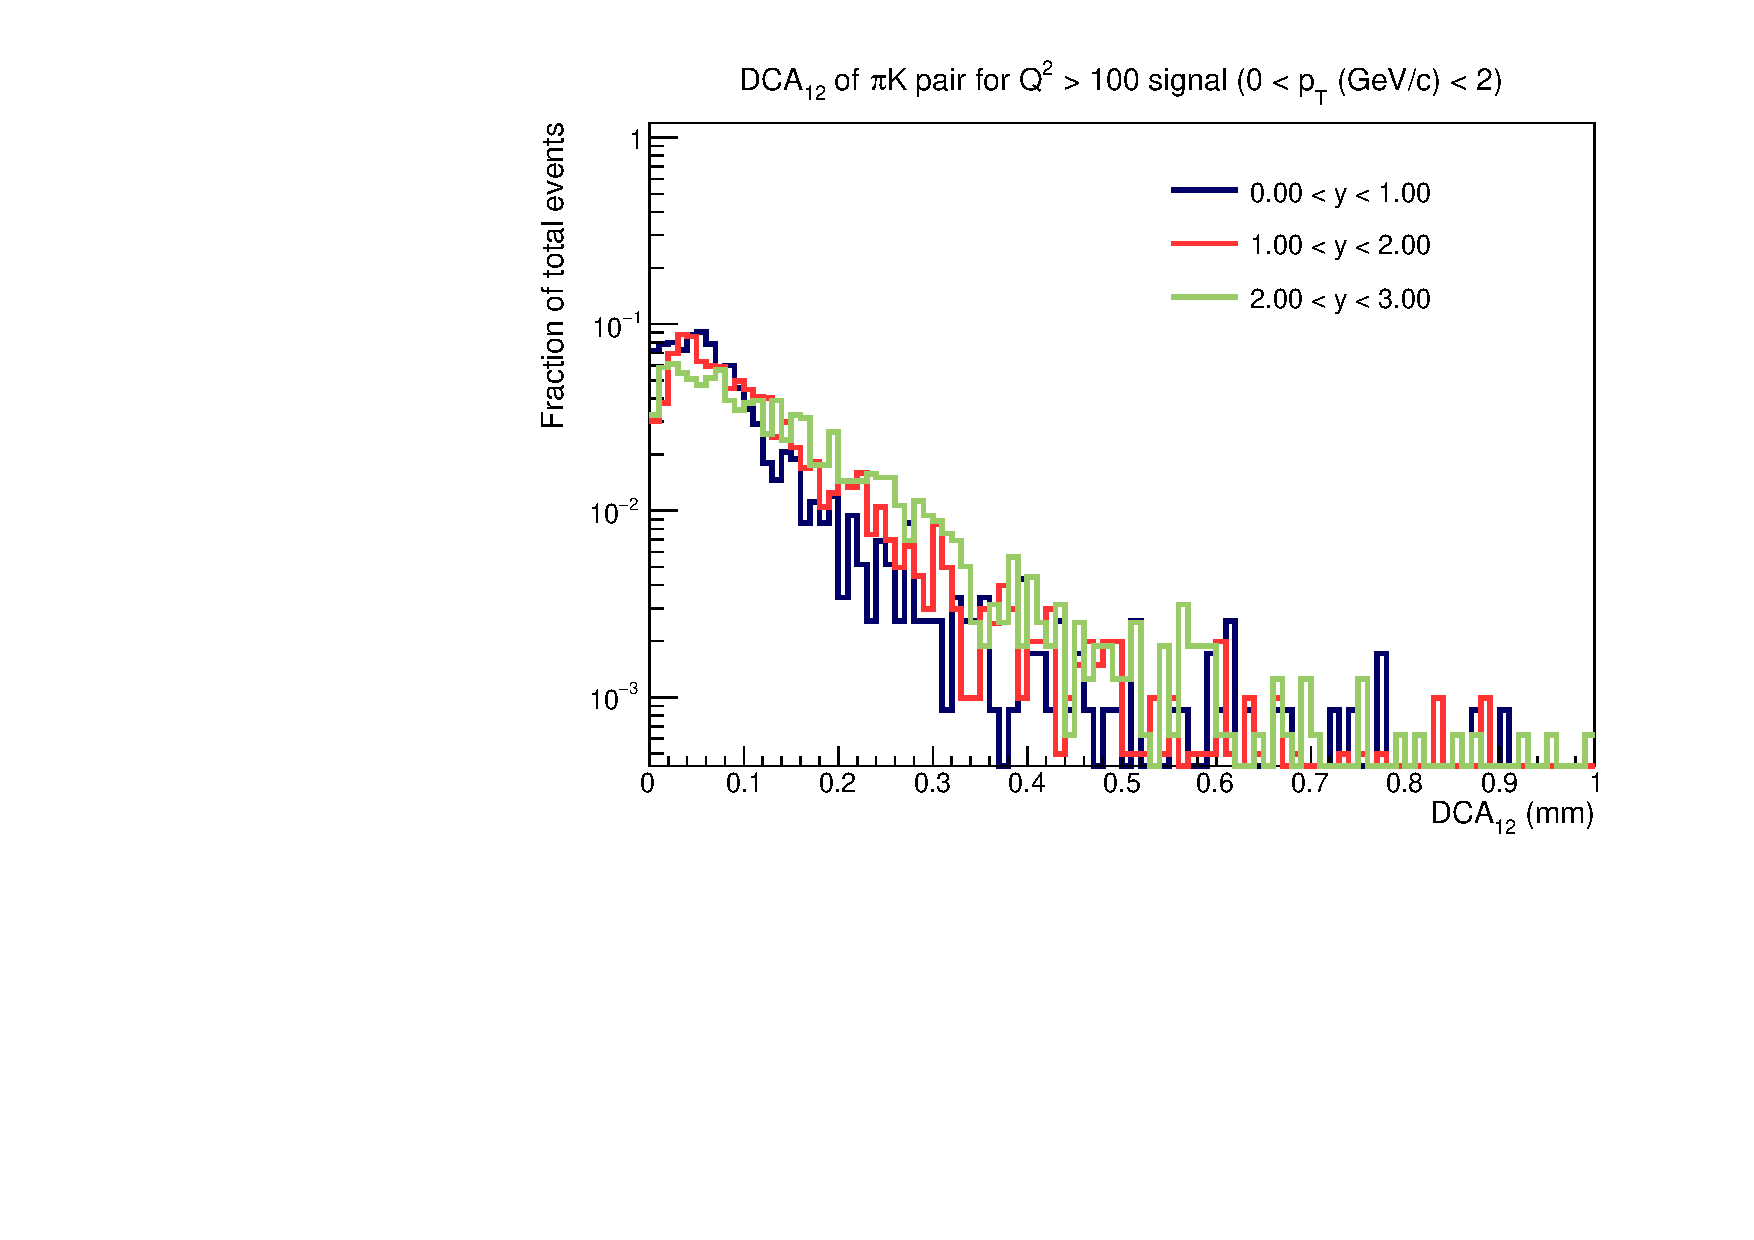
\includegraphics[width=0.55\linewidth]{gallery/D0_topology/DCA12_by_y.pdf}
    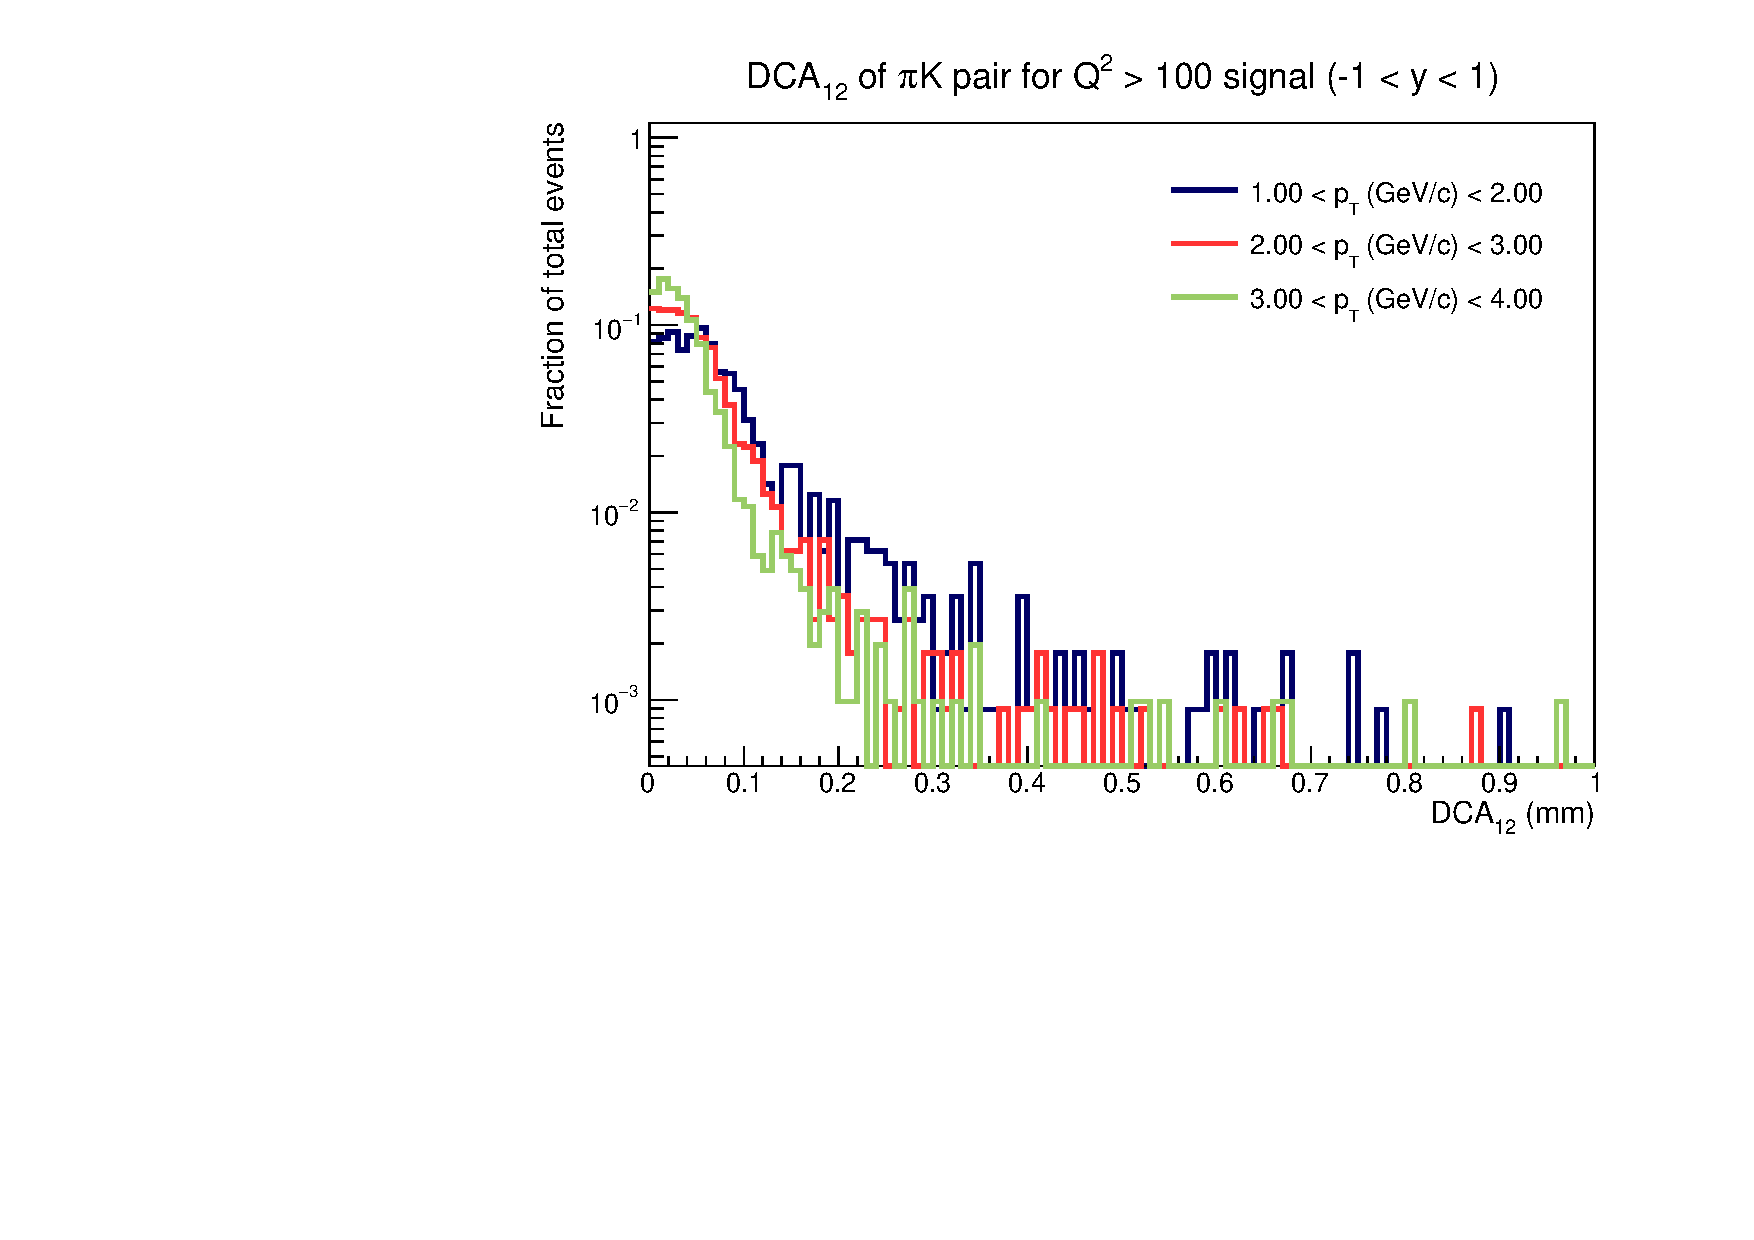
\includegraphics[width=0.55\linewidth]{gallery/D0_topology/DCA12_by_pt.pdf}
    \caption{Examples of the $y$- and $p_T$-dependence of $\text{DCA}_{12}$ of reconstructed $D^0$-mesons in simulated $Q^2>100~\text{GeV}^2$ $ep$ collisions. The top plot compares distributions in various $y$ ranges for $0<p_T<2$ GeV/c, and the bottom plot compares distributions in various $p_T$ ranges for $-1<y<1$.}
    \label{f.top_by_y_pt}
\end{figure}
%

With these effects in mind, we examined the topological variables for reconstructed $D^0$-mesons from simulated $ep$ collisions in different slices of $y$ and $p_T$.  Fig. \ref{f.top_by_y_pt} illustrates these kinematic dependences for the $\text{DCA}_{12}$. As expected, we observe that forward $y$ (green line in the top plot) and low $p_T$ (blue line in the bottom plot) result in wider distributions, which indicate a larger degree of uncertainty in the true value of the topological variables in these regions. This suggests worsening reconstruction performance as we move toward forward $y$ low $p_T$. The distributions for ${\rm DCA_{D0}}$, ${\rm DCA_{\pi}}$, ${\rm DCA_{K}}$, and $\theta$ exhibit the same trends, as expected.

%
\begin{figure}[h!]
    \centering
    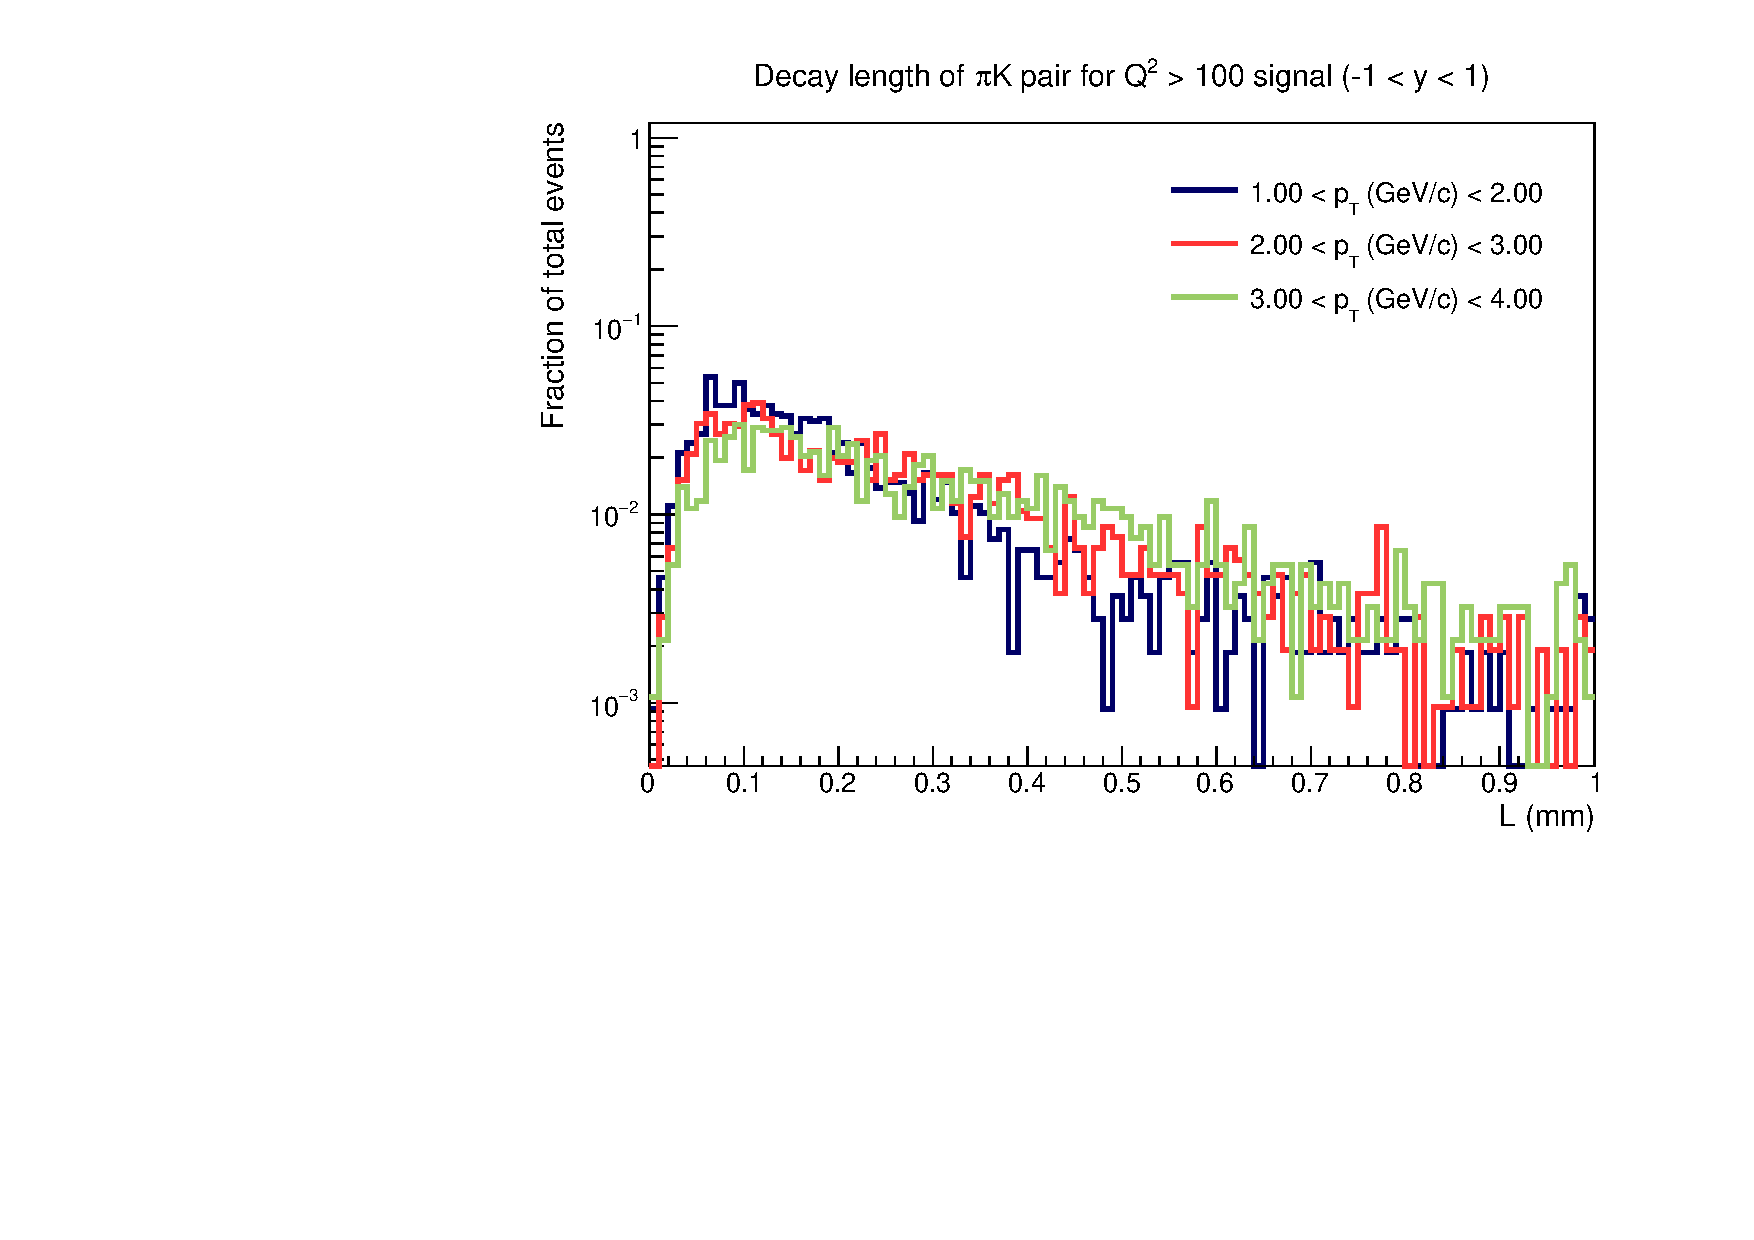
\includegraphics[width=0.55\linewidth]{gallery/D0_topology/dl_pt.pdf}
    \caption{$p_T$-dependence of the decay length of reconstructed $D^0$-mesons in simulated $Q^2>100~\text{GeV}^2$ $ep$ collisions, comparing various $p_T$ ranges for $01<y<1$.}
    \label{f.dl}
\end{figure}
%
As shown in Fig. \ref{f.dl}, the decay length exhibits the opposite dependence on $p_T$, in which the distribution seem wider at high $p_T$ (green line). This can be explained by higher-$p_T$ $D^0$-mesons traveling farther before decaying, which results in the decay length distribution peaking at a higher value.

%
\begin{figure}[h!]
    \centering
    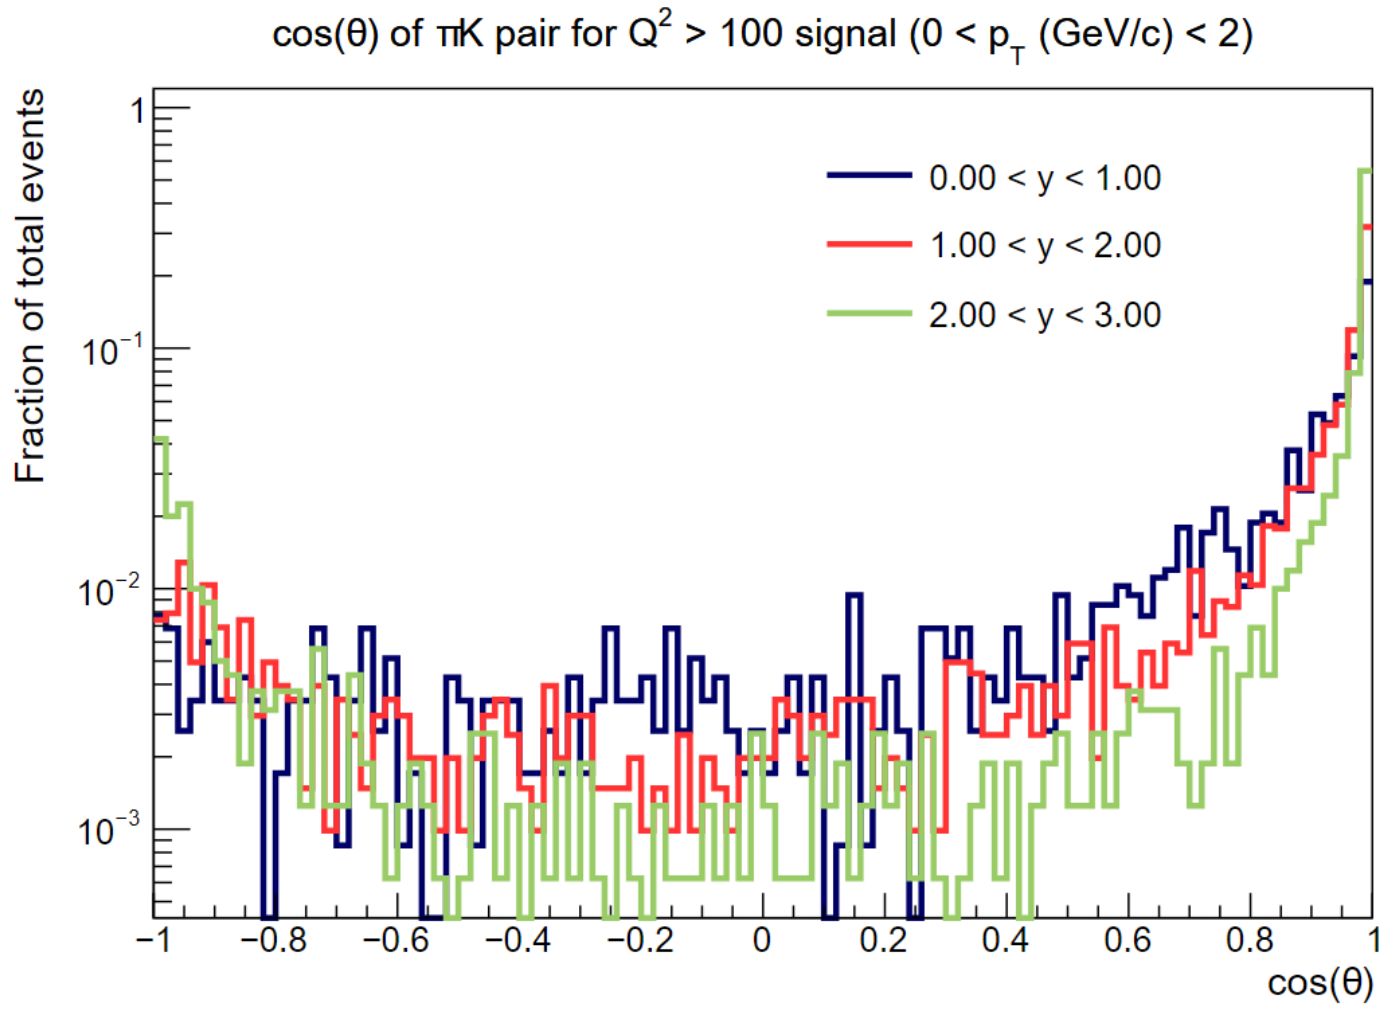
\includegraphics[width=0.55\linewidth]{gallery/D0_topology/costheta_y.png}
    \caption{$y$-dependence of $\cos{\theta}$ of reconstructed $D^0$-mesons in simulated $Q^2>100~\text{GeV}^2$ $ep$ collisions, comparing various $y$ ranges for $0<p_T<2$ GeV/c.}
    \label{f.costheta}
\end{figure}
%
When examining the topological distributions, we found that the deterioration of reconstruction performance at forward $y$ is especially apparent in plots of $\cos{\theta}$, as shown in Fig. \ref{f.costheta}. We expect the $\theta$ distribution to be centered around 0, which corresponds to the peak at $\cos{\theta}=1$. However, at forward $y$ (green line), we notice another peak at $\cos{\theta}=-1$. This second peak corresponds to $D^0$-mesons with a momentum vector $\overrightarrow{P}$ reconstructed antiparallel to its expected direction of travel, which is un-physical. This observation points toward the need for further improvements in reconstruction at forward rapidity.

% %
% \begin{figure}[hb!]
%     \centering
%     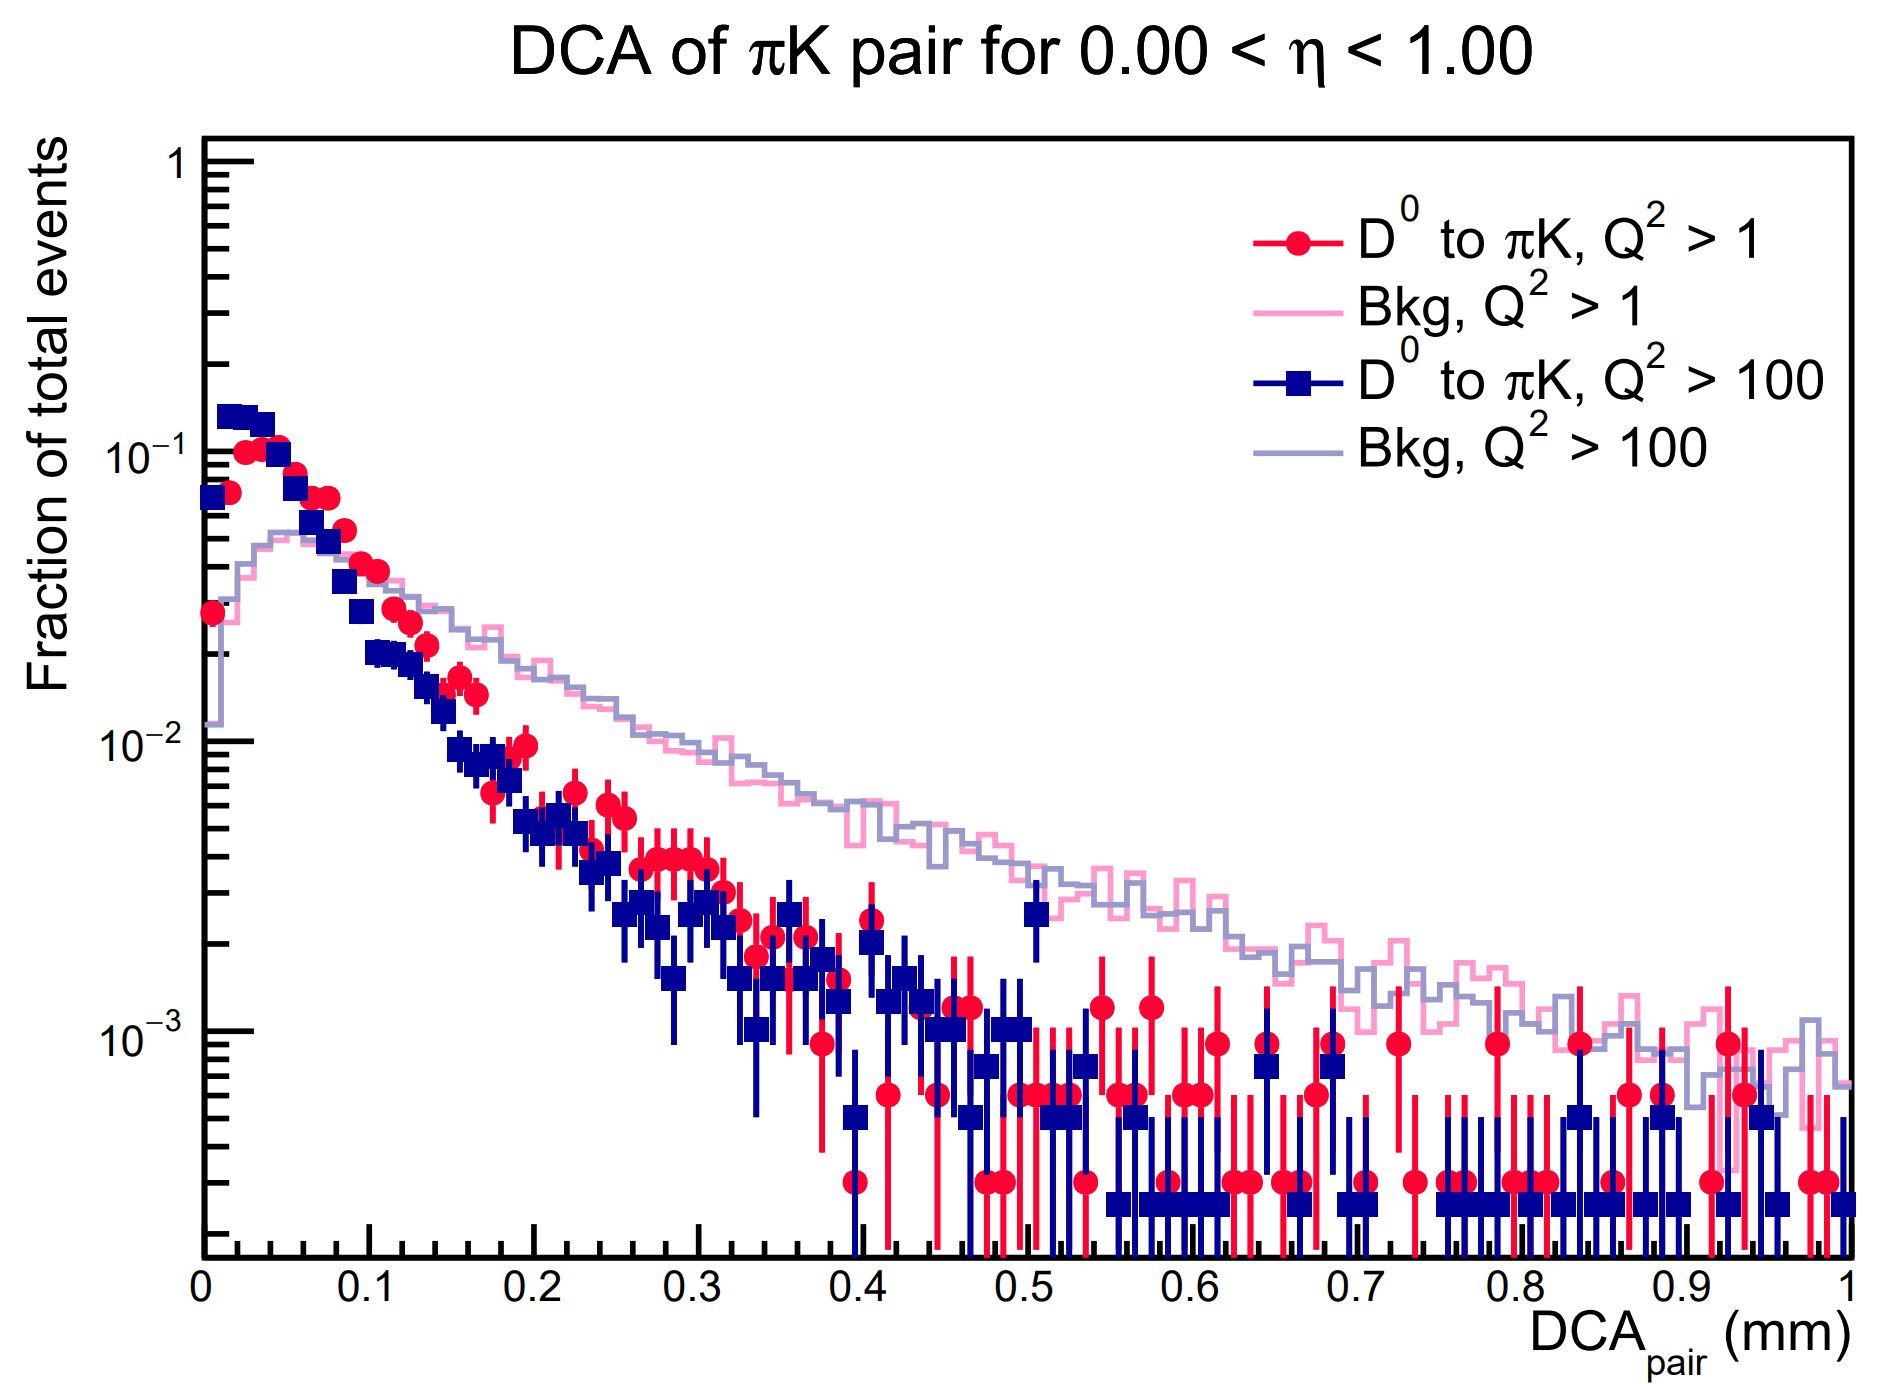
\includegraphics[width=0.45\linewidth]{gallery/D0_topology/DCA_Q2_dep.png}
%     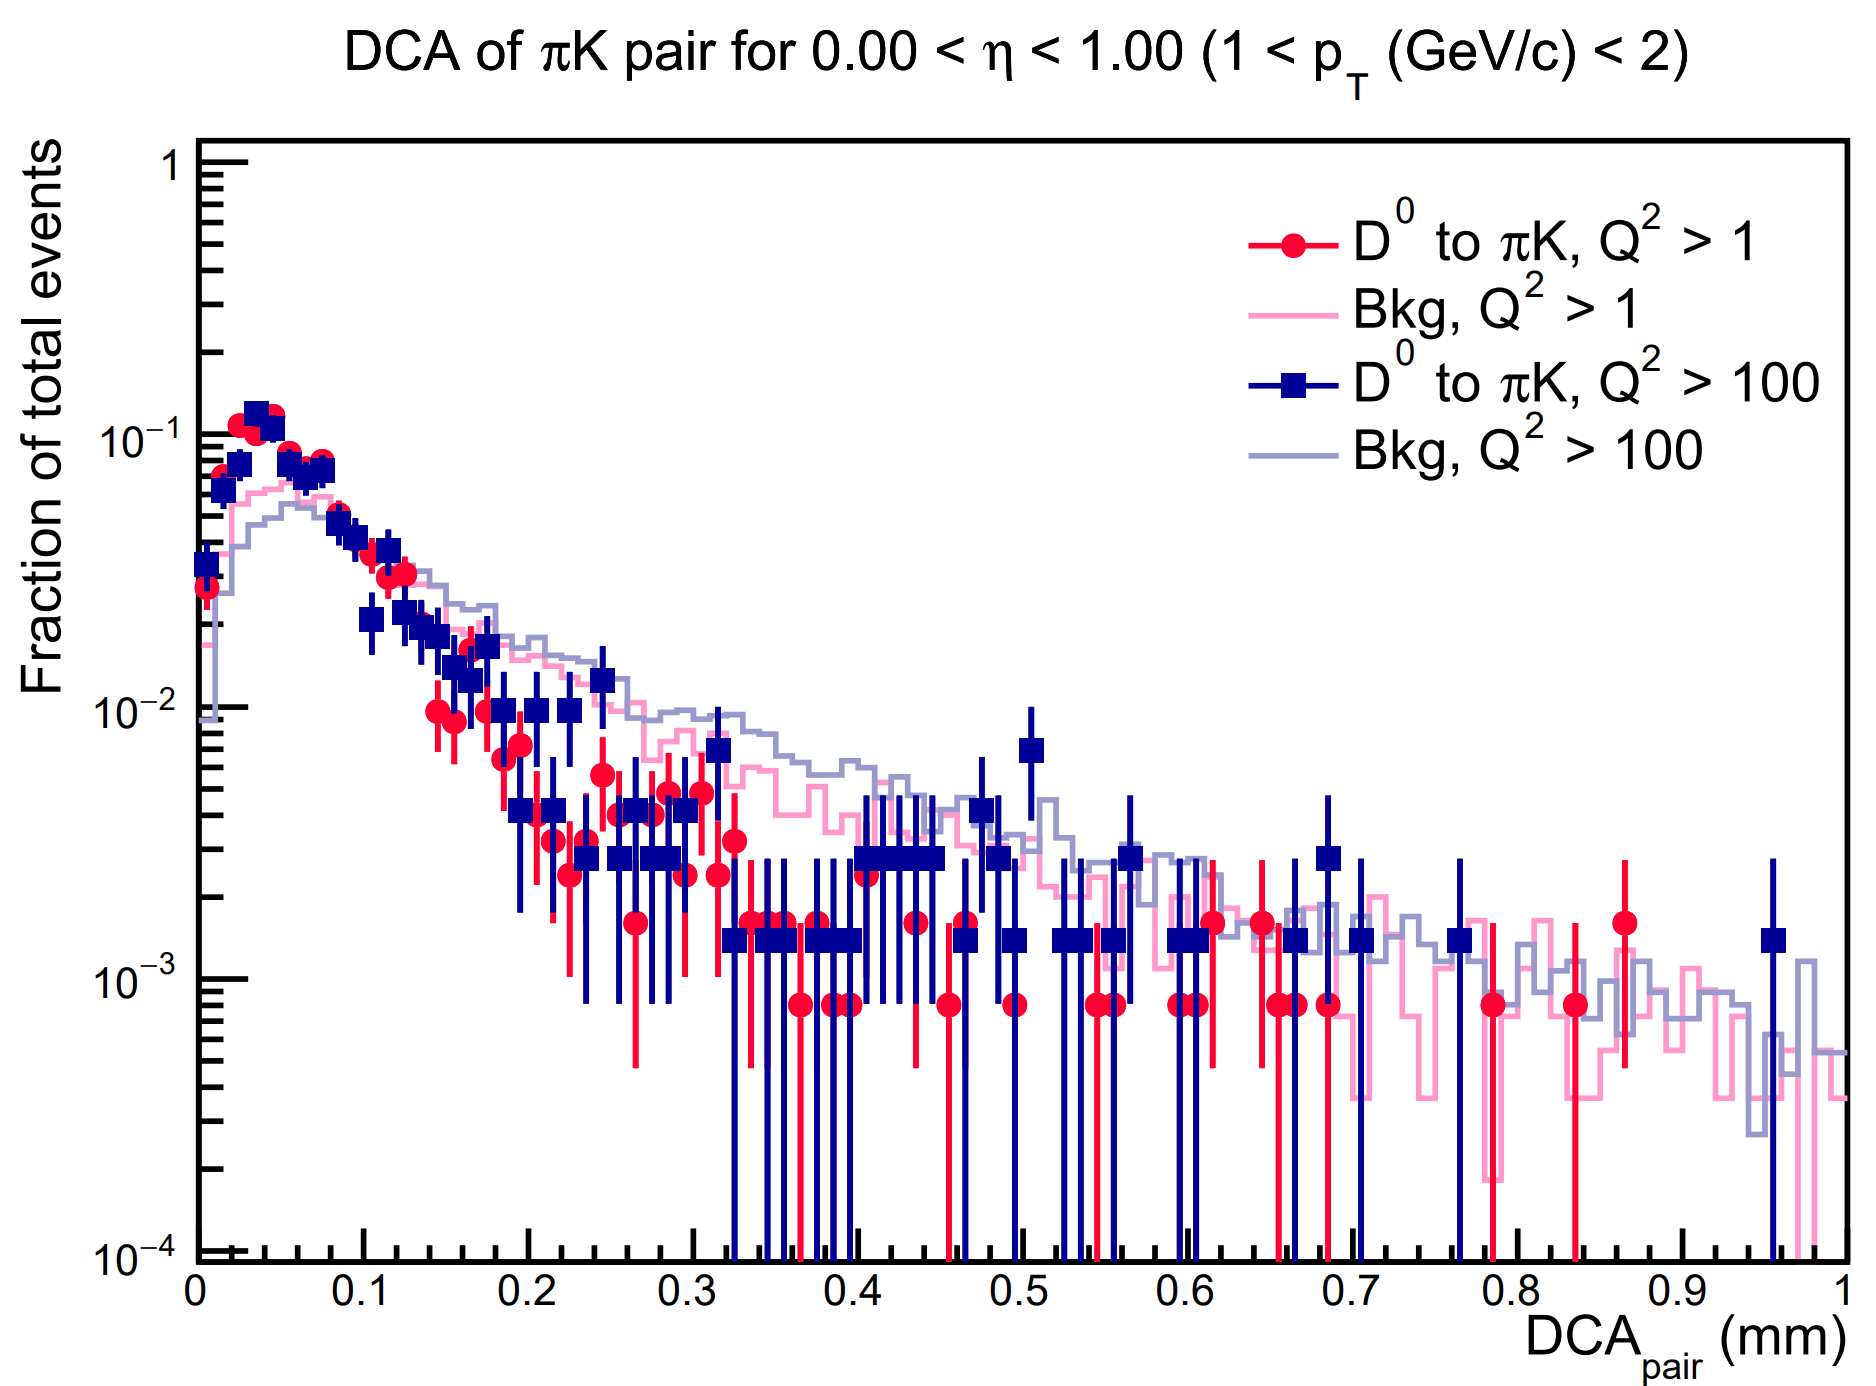
\includegraphics[width=0.45\linewidth]{gallery/D0_topology/DCA_Q2_dep_removed.png}
%     \caption{Comparison of $\text{DCA}_{D^0}$ distributions of $D^0$ signal and background candidates between $Q^2>1~\text{GeV}^2$ (red) and $Q^2>100~\text{GeV}^2$ (blue) $ep$ collisions, in the range $0<\eta<1$. The left plot shows the $p_T$-integrated distributions, and the right plot shows the distributions for the slice $1<p_T<2$.}
%     \label{f.top_by_y_pt}
% \end{figure}
% %

% %
% \begin{figure}[h!]
%     \centering
%     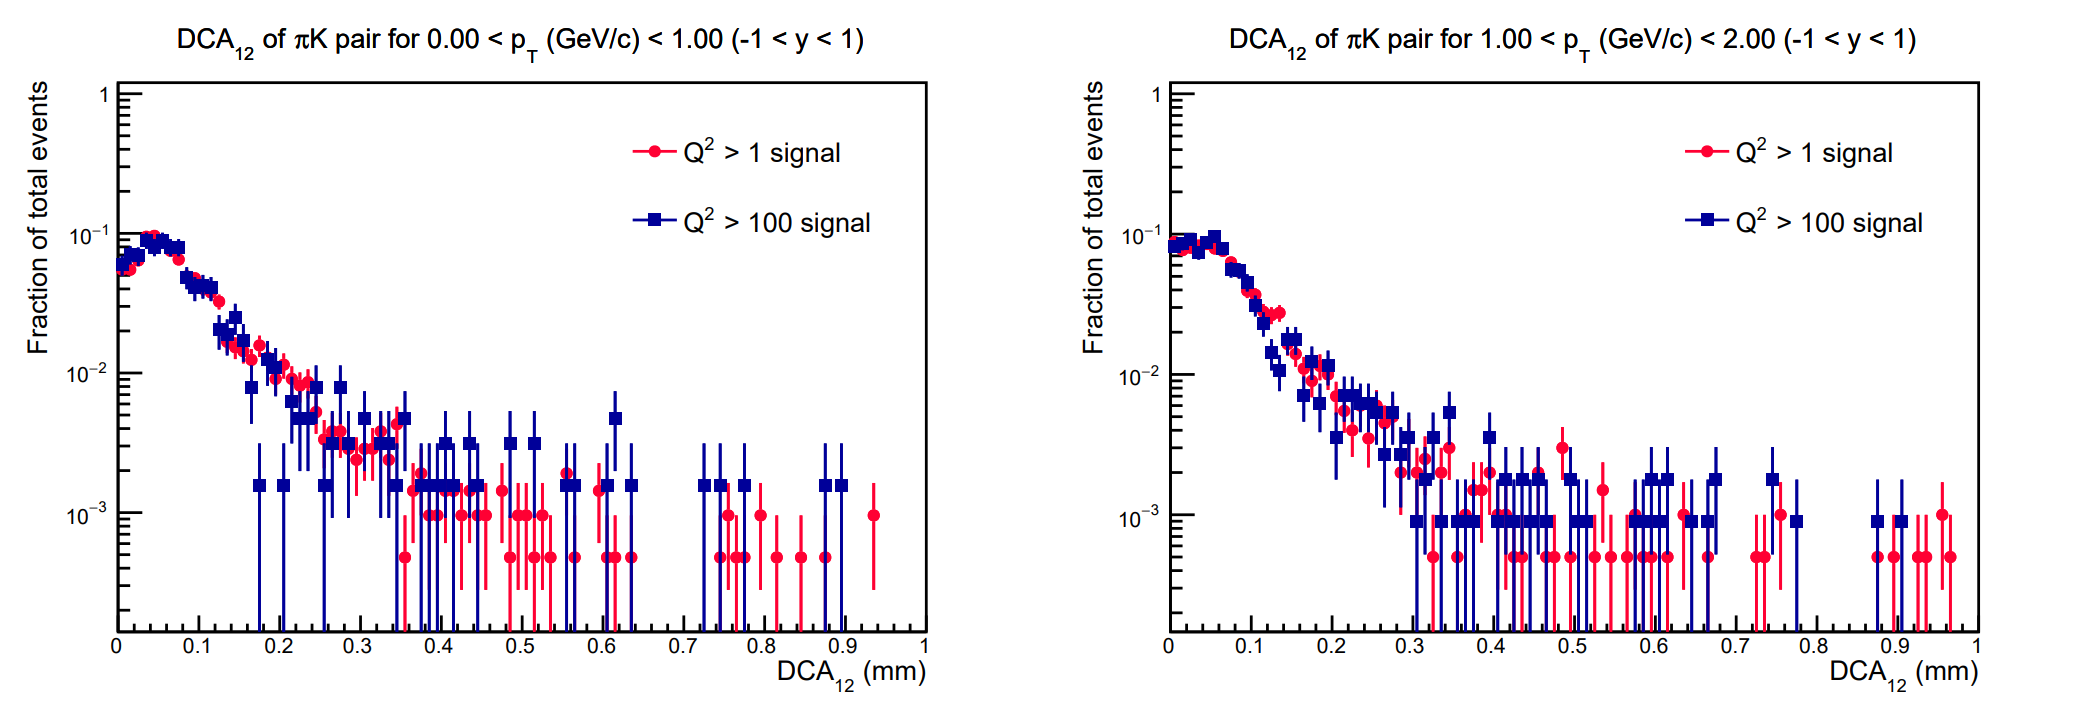
\includegraphics[width=0.95\linewidth]{gallery/D0_topology/DCA12_slices_1.png}
%     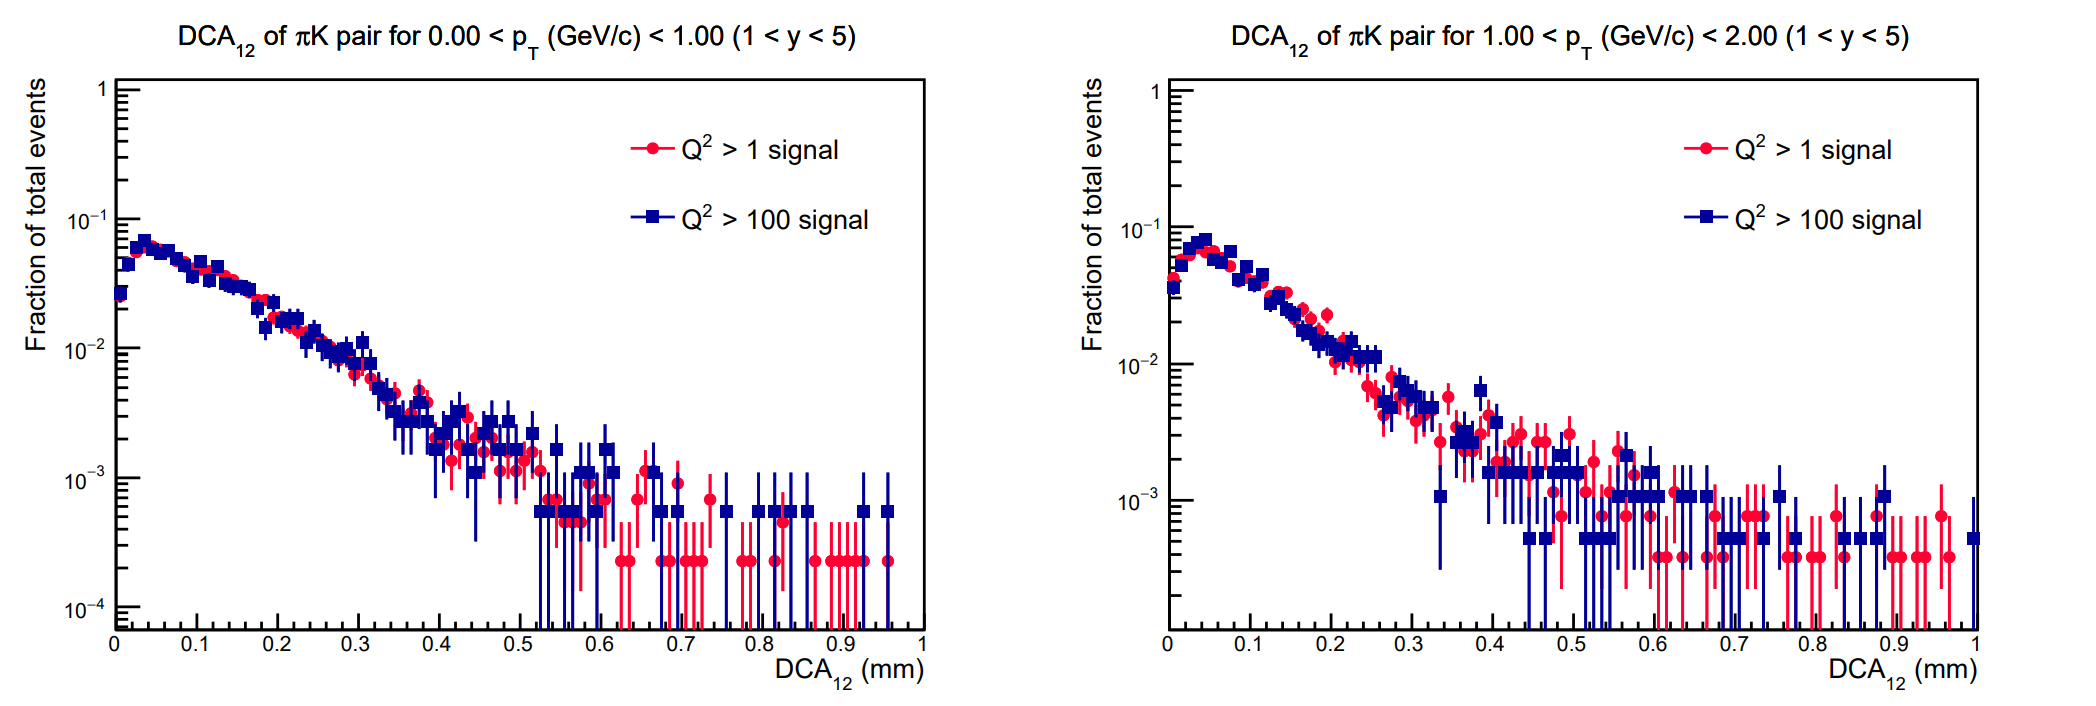
\includegraphics[width=0.95\linewidth]{gallery/D0_topology/DCA12_slices_2.png}
%     \caption{Comparison of $\text{DCA}_{12}$ distributions between $Q^2>1~\text{GeV}^2$ (red circles) and $Q^2>100~\text{GeV}^2$ (blue squares) $ep$ collisions for $D^0$ signal candidates in various slices of $y$ and $p_T$. (Can consider using a different top. var. as an example.)}
%     \label{f.top_by_Q2}
% \end{figure}
% %
%
\begin{figure}[h!]
    \centering
    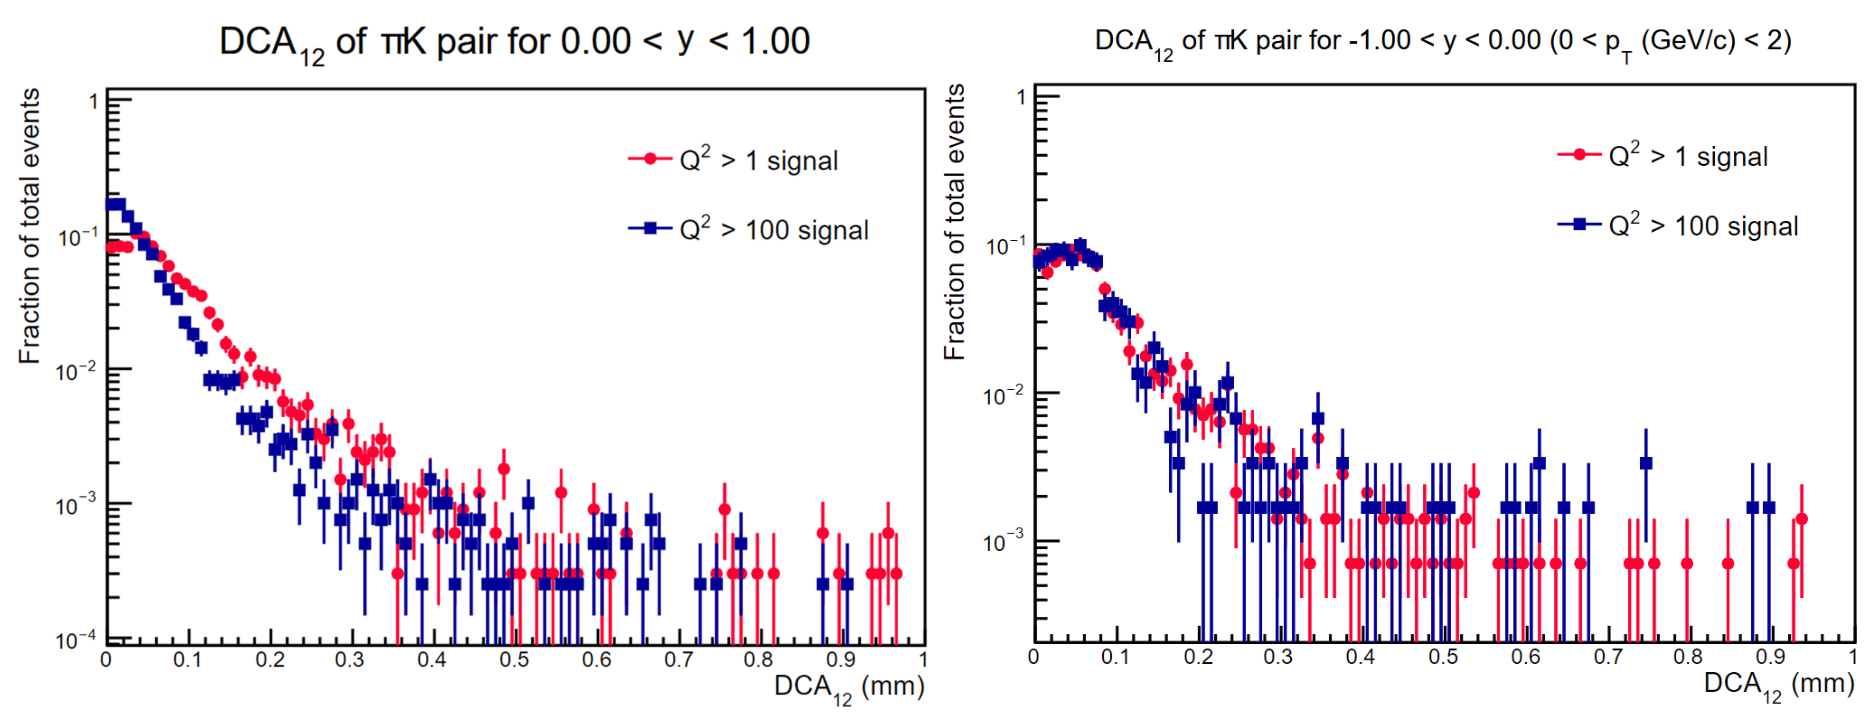
\includegraphics[width=0.9\linewidth]{gallery/D0_topology/top_q2.png}
    \caption{Comparison of $\text{DCA}_{12}$ distributions between $Q^2>1~\text{GeV}^2$ and $Q^2>100~\text{GeV}^2$$ep$ collisions for reconstructed $D^0$-mesons with any $p_T$ (left) vs. with $0<p_T<2$ GeV/c, both at mid-$y$.}
    \label{f.top_by_Q2}
\end{figure}
%
One last kinematic consideration concerns $Q^2$, defined in Ch. \ref{sec.bkg_emu}, which is the square of the four-momentum transferred in the $ep$ collision. The value of $Q^2$ determines how much energy is available for all the particles produced in the interaction. In Fig. \ref{f.top_by_y_pt}-\ref{f.costheta}, we have presented results for collisions with high four-momentum transfer, $Q^2>100~{\rm GeV^2}$. However, experiments at the EIC will also span a wide range of $Q^2$, and $ep$ collisions generally look different at various energy levels. For example, high $Q^2$ collisions tend to produce more $D^0$-mesons with large $p_T$ while low $Q^2$ collisions produce more particles with low $p_T$. Thus, we can expect the $Q^2$-dependence of topological variables to follow the same trends as their $p_T$-dependence. To examine the effects of $Q^2$ on the $D^0\rightarrow\pi+K$ topology, we compare the topological distributions of $D^0$-mesons produced in $Q^2>1~{\rm GeV^2}$ and $Q^2>100~{\rm GeV^2}$ collisions. Fig. \ref{f.top_by_Q2} shows these distributions for ${\rm DCA_{12}}$.

In the left plot, which includes all $D^0$-mesons with any $p_T$, we find that the ${\rm DCA_{12}}$ distribution is wider for $Q^2>1~{\rm GeV^2}$ collisions compared to the higher energy $Q^2>100~{\rm GeV^2}$ collisions. However, due to the correlation between $Q^2$ and $p_T$, the dependence on $Q^2$ is removed when restricting to individual $p_T$ slices. As we see in the right plot of Fig. \ref{f.top_by_Q2}, which only includes $D^0$-mesons with $0<p_T<2~{\rm GeV/c}$, there are no significant differences between the topological distributions for $Q^2>1~\text{GeV}^2$ and $Q^2>100~\text{GeV}^2$ collisions.

%--------------------------------------------------------
\section{Strategy for $D^0$ signal-background separation with topological cuts}
\label{sec.d0_strategy}

%
\begin{figure}[h!]
    \centering
    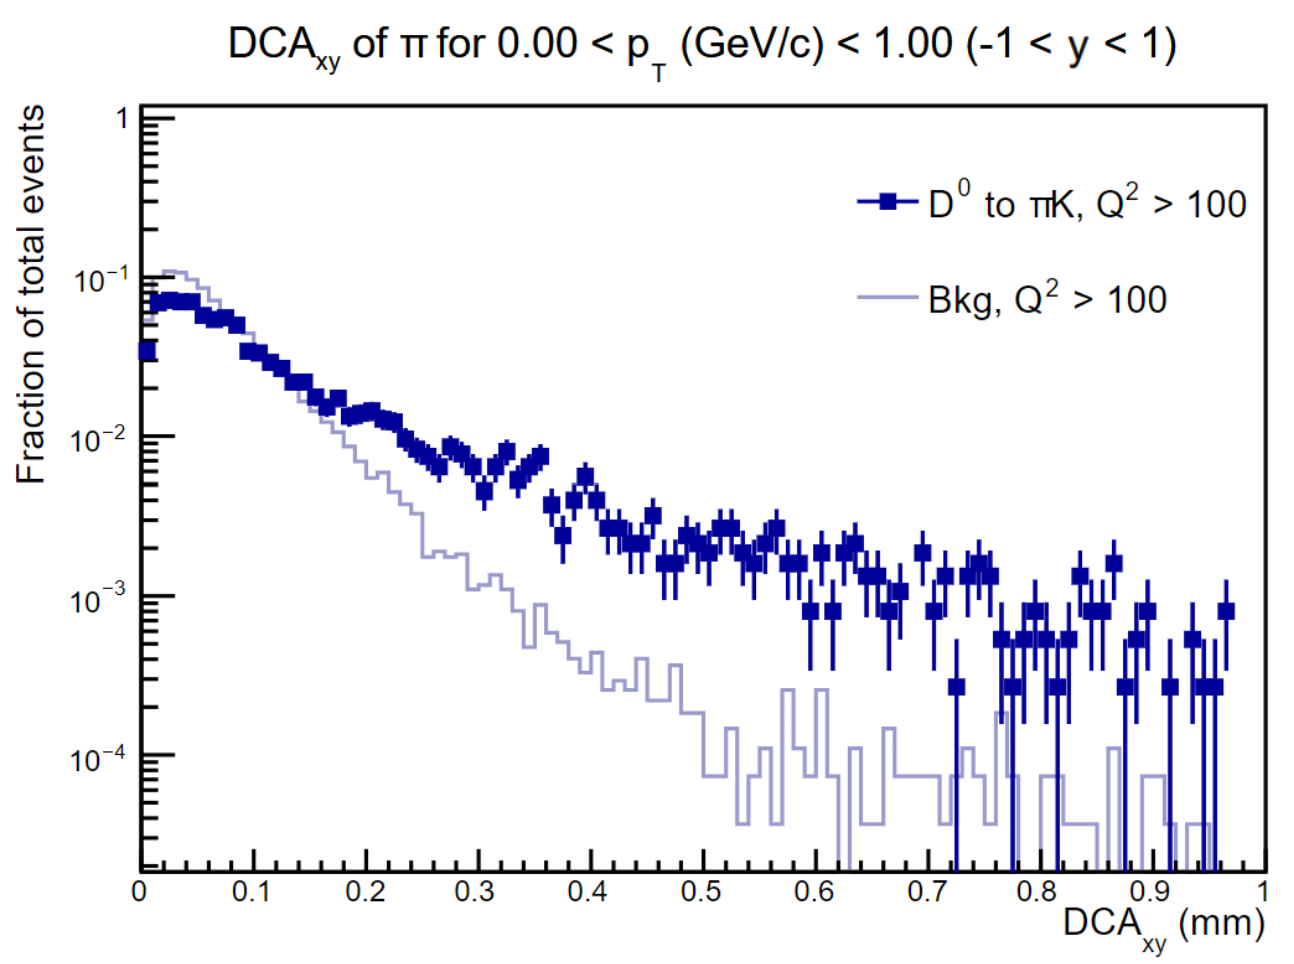
\includegraphics[width=0.6\linewidth]{gallery/D0_topology/top_cut.png}
    \caption{Example comparison of ${\text{DCA}}_{{\rm \pi}(xy)}$ distributions for reconstructed $D^0$-mesons (discrete markers) and background (line).}
    \label{f.top_cut}
\end{figure}
%
Our goal is to use the shapes of the topological distributions, which generally look different for true $D^0$-mesons (signal) and for the background. Fig. \ref{f.top_cut} shows an example comparing the signal and background distributions for ${\text{DCA}}_{{\rm \pi}(xy)}$. We would like to select some cut value $x$, such that we accept all candidates with ${\text{DCA}}_{{\rm \pi}(xy)}<x$ as signal and reject all candidates with ${\text{DCA}}_{{\rm \pi}(xy)}>x$. In practice, we will always end up accepting some mixture of signal and background candidates. However, with the help of machine learning, we can look for the most optimal cut that maximizes the number of signal candidates while minimizing the number of background candidates.

%
\begin{table}[h!]
    \centering
    \begin{tabular}{c|c|c}
                & $-1<y<1$ & $1<y<3$ \\
                \hline
    $1<p_T<2~{\rm GeV/c}$   & mid-$y$, low $p_T$ & forward $y$, low $p_T$ \\
    $2<p_T<3~{\rm GeV/c}$   & mid-$y$, high $p_T$ & forward $y$, high $p_T$ \\
    \end{tabular}
    \caption{Kinematic slices in $y$ and $p_T$ of the $D^0$ considered in this analysis.}
    \label{tab.kinematics}
\end{table}
%
In the previous section, Ch. \ref{sec.top_y_pt_slices}, we have seen that the $D^0\rightarrow\pi+K$ topology depends significantly on both $y$ and $p_T$. As a result, the set of topological cuts that gives the best signal-and-background separation for one $y$ and $p_T$ range may not perform well for other ranges. Therefore, we optimize the separation of $D^0$ signals from background for individual slices of $y$ and $p_T$. Specifically, we divide the data into the 4 kinematic categories in Table \ref{tab.kinematics}.

We do not include backward rapidity $y<-1$ and $p_T>3$ due to these regions having low statistics (see Fig. \ref{f.y_pT}), meaning that the regions are sparsely populated and thus have large statistical uncertainties. Given that we consider small slices in $p_T$. the topological distributions are independent with respect to $Q^2$. Thus, we analyze all particles for $Q^2>1~\text{GeV}^2$, which includes low and high energy collisions. In Ch. \ref{ch.results}, we will discuss the optimization of topological cuts in these various kinematic regions using machine learning.